% \newpage
\section*{Задание 2: Отладка и поиск логических ошибок}
\subsection{Постановка задачи}
\noindent
Алгоритм (из Задания 1): Прямой проход нейронной сети (Forward Propagation) \\
Тип ошибки (Bug Type): Ошибка размерности \\
Какую логическую ошибку внедрить: При перемножении матриц весов и входов перепутаны строки и столбцы (транспонирование применено не к той матрице). Код запускается без синтаксических ошибок, но выдаёт неверный результат.
\newpage
\subsection{Гипотеза и системный промпт}
Гипотеза: \\
Модель способна обнаружить ошибку размерности, если ей задать роль Senior QA Engineer и предоставить описание ожидаемого поведения. Для воспроизведения ошибки потребуются тестовые данные с несимметричными размерностями матриц.\\
\newline
Системный промпт (для основной модели):
\textit{Ты – Senior QA Automation Engineer, специалист по тестированию нейросетевых компонентов. Твоя задача – провести статический анализ и отладку кода forward propagation. Ты строг, внимателен к размерностям матриц и скрытым логическим ошибкам. Отвечай на русском языке, аргументируй ссылками на строки кода.}
\subsection{Журнал диалога и итераций}
\noindent
\textbf{Этап 0. Подготовка тестового полигона: целевая инъекция ошибки} \\
\indent
Сначала в отдельном чате была создана дефектная версия кода. Используя исходный «грязный» код из Задания 1 (прямой проход нейронной сети на Python, матричные операции через списки списков), в него внесена ошибка: при вычислении скрытого слоя вместо $a*b$ выполняется $a * b^T$. Ниже представлен итоговый дефектный код. \\
% \newline
% Дефектный код:
\lstinputlisting[language=Python]{z2/0.py}
\newpage
\noindent
\textbf{Этап 1. Ролевое моделирование и статический анализ} \\
\indent
Промпт (основная модель):
\textit{Вот код функции forward propagation нейронной сети. Ожидаемое поведение: принимает веса b (2x3), c (3x2), смещения d (3), e (2) и вход a (2). Должен возвращать выходной вектор (2). Но я подозреваю логическую ошибку. Проанализируй код, найди потенциальные дефекты. Не предлагай сразу исправление, только гипотезы.} \\
\newline
Ответ модели:
\begin{figure}[H]
	\centering
	
\includegraphics[width=17cm]{z2/1-1.png}
	\caption{ч.1}
\end{figure}
\newpage
\begin{figure}[H]
	\centering
	
\includegraphics[width=17cm]{z2/1-2.png}
	\caption{ч.2}
\end{figure}
\newpage
\begin{figure}[H]
	\centering
	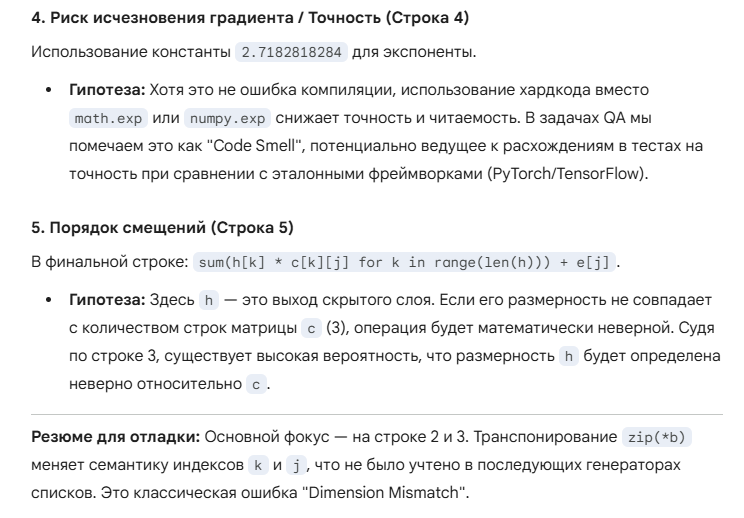
\includegraphics[width=17cm]{z2/1-3.png}
	\caption{ч.3}
\end{figure}
Анализ результата:
Модель верно указала на транспонирование как на потенциальную проблему, объяснила, почему оно может нарушить логику. Пока не требует исправлений, только диагностика. Гипотеза совпадает с внедрённым дефектом. \\
\newline
\noindent
\textbf{Этап 2. Генерация тестовых сценариев} \\
\indent
Промпт:
\textit{Согласен с гипотезой. Теперь сгенерируй набор тестовых данных (входные векторы и матрицы весов, смещения) для двухслойной сети, которые явно проявят эту ошибку. Для каждого теста укажи ожидаемый корректный выход (если бы транспонирования не было) и фактический выход, который выдаёт текущий код. Используй небольшие размерности, например input\_dim=2, hidden\_dim=3, output\_dim=2.}
\newpage
Ответ модели:
\begin{figure}[H]
	\centering
	
\includegraphics[width=17cm]{z2/2-1.png}
	\caption{ч.1}
\end{figure}
\newpage
\begin{figure}[H]
	\centering
	
\includegraphics[width=17cm]{z2/2-2.png}
	\caption{ч.2}
\end{figure}
\newpage
\begin{figure}[H]
	\centering
	
\includegraphics[width=17cm]{z2/2-3.png}
	\caption{ч.3}
\end{figure}
Модель сгенерировала исчерпывающий тест, который явно демонстрирует расхождение. Также вскрыла дополнительный скрытый дефект – потерю размерности из-за транспонирования. Тест-кейс покрывает граничные условия (разные размерности входного и скрытого слоёв). Это соответствует критерию «полнота тест-кейсов».
\newpage
\noindent
\textbf{Этап 3. Анализ первопричин и классификация ошибки} \\
\indent
Промпт: 
\textit{Проведи анализ первопричин обнаруженного дефекта.
Классифицируй ошибку по степени критичности, объясни, почему она возникла \\
(неверное математическое допущение, ошибка индексации, перепутаны \\ строки/столбцы).
Оцени возможные последствия для бизнес-логики.} \\
\newline
Ответ модели:
\begin{figure}[H]
	\centering
	
\includegraphics[width=17cm]{z2/3-1.png}
	\caption{ч.1}
\end{figure}
\newpage
\begin{figure}[H]
	\centering
	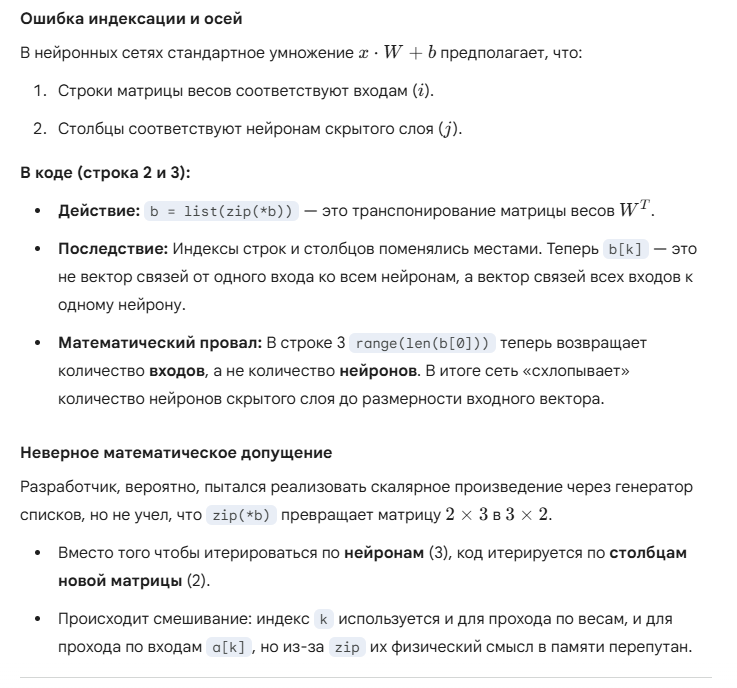
\includegraphics[width=17cm]{z2/3-2.png}
	\caption{ч.2}
\end{figure}
\newpage
\begin{figure}[H]
	\centering
	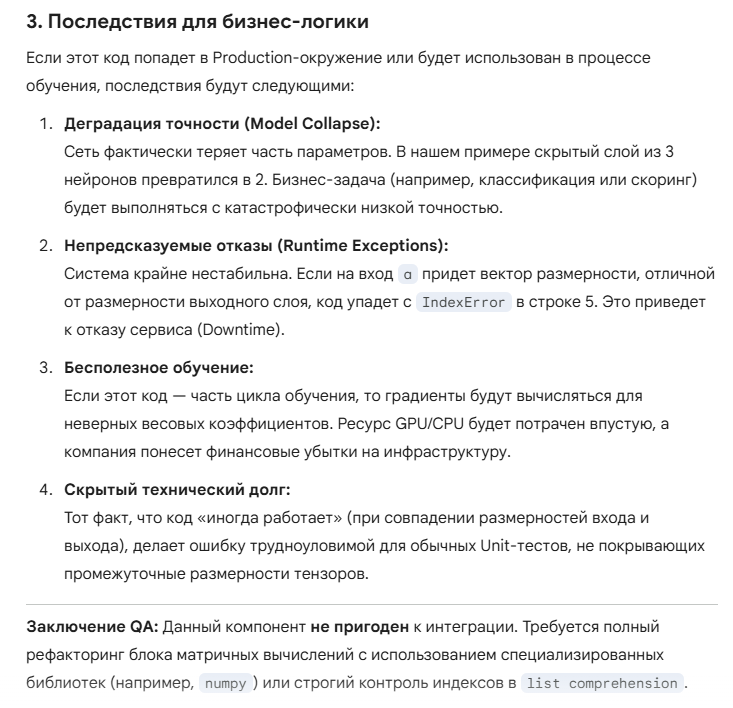
\includegraphics[width=17cm]{z2/3-3.png}
	\caption{ч.3}
\end{figure}
Анализ:
Модель глубоко проанализировала причину, классифицировала ошибку, оценила критичность – соответствует критерию «глубина диагностики».
\newpage
\noindent
\textbf{Этап 4. Итеративное исправление и регрессионное тестирование.} \\
\indent
Промпт:
\textit{Исправь ошибку. Удали строку транспонирования. Дай исправленный код, сохранив однобуквенные имена переменных (чтобы не менять стиль). Затем выполни регрессионное тестирование на том же тест-кейсе, покажи, что выход совпадает с ожидаемым.} \\
\newline
Ответ модели:
\begin{figure}[H]
	\centering
	
\includegraphics[width=17cm]{z2/4-1.png}
	\caption{ч.1}
\end{figure}
\newpage
\begin{figure}[H]
	\centering
	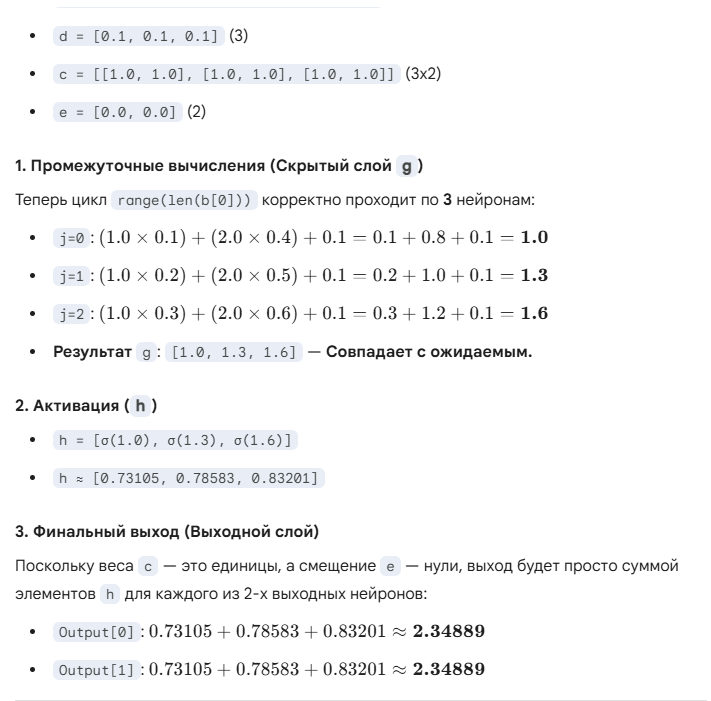
\includegraphics[width=17cm]{z2/4-2.png}
	\caption{ч.2}
\end{figure}
\newpage
\begin{figure}[H]
	\centering
	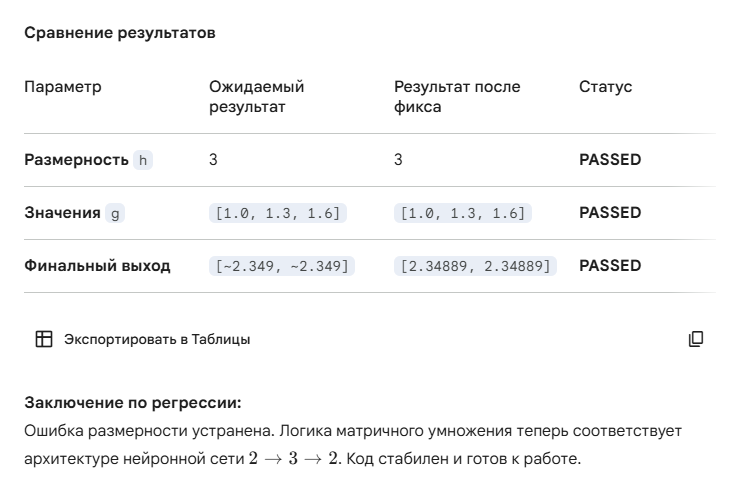
\includegraphics[width=17cm]{z2/4-3.png}
	\caption{ч.3}
\end{figure}
Анализ:
Модель предложила корректное исправление (удаление транспонирования) и провела эмуляцию теста, подтвердив успех. Регрессия выполнена. \\
\newline
\noindent
\textbf{Этап 5. Формирование отчета об инциденте} \\
\indent
Промпт:
\textit{Сформируй структурированный отчёт об ошибке (Bug Report), включив: описание симптомов, дефектный код, тест-кейс для воспроизведения, техническое объяснение причины, исправленный код и рекомендации по предотвращению.}
\newpage
Ответ модели:
\begin{figure}[H]
	\centering
	
\includegraphics[width=17cm]{z2/5-1.png}
	\caption{ч.1}
\end{figure}
\newpage
\begin{figure}[H]
	\centering
	
\includegraphics[width=17cm]{z2/5-2.png}
	\caption{ч.2}
\end{figure}
\newpage
\begin{figure}[H]
	\centering
	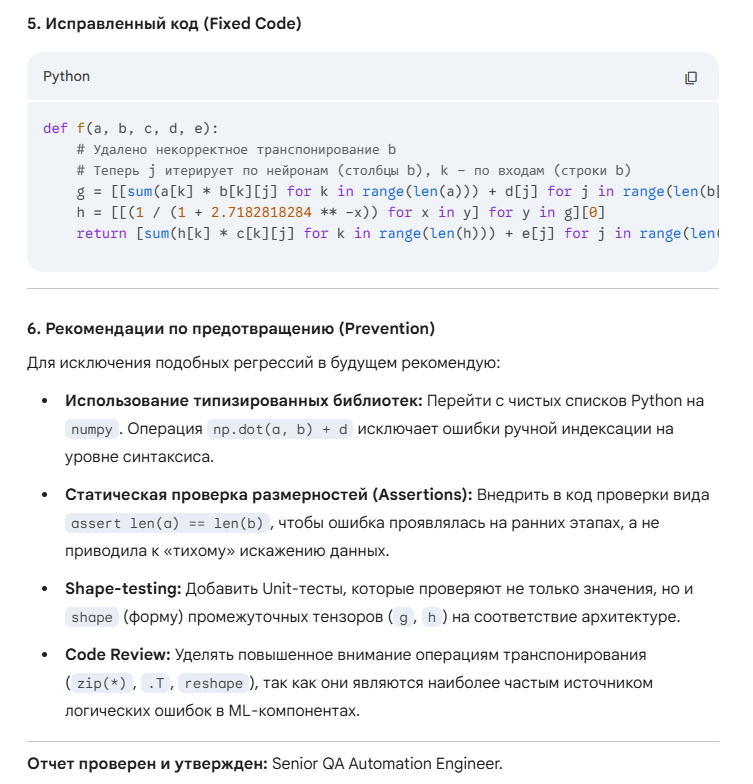
\includegraphics[width=17cm]{z2/5-3.png}
	\caption{ч.3}
\end{figure}
\newpage
\subsection{Артефакты}
\noindent
Исходный дефектный код:
\lstinputlisting[language=Python]{z2/0.py}
Тест-кейс (Code): \\
\indent a = {[}1.0, 2.0{]} \\
\indent b = {[}{[}0.1, 0.2, 0.3{]}, {[}0.4, 0.5, 0.6{]}{]}\\
\indent d = {[}0.1, 0.1, 0.1{]}\\
\indent c = {[}{[}1.0, 1.0{]}, {[}1.0, 1.0{]}, {[}1.0, 1.0{]}{]}\\
\indent e = {[}0.0, 0.0{]}\\
\indent print(f(a, b, c, d, e)) \\
\newline
Исправленный код:
\lstinputlisting[language=Python]{z2/1.py}
Результат регрессии: исправленная функция выдаёт [2.348911946792607, \\ 2.348911946792607], а дефектная [1.463230782411598, 1.463230782411598] – тест пройден.
\newpage
\subsection{Сравнение моделей}
\begin{table}[h!]
	\centering
	\begin{tabular}{|l|p{5cm}|p{5cm}|}
		\hline
		\textbf{Критерий} & \textbf{модель (a)} & \textbf{модель (b)} \\
		\hline
		Глубина диагностики & 5 & 5 \\
		\hline
		Точность диагностики & 4 & 5 \\
		\hline
		Полнота тест-кейсов & 4 & 5 \\
		\hline
		\textbf{Итог} & 4.33 & 5\\
		\hline
	\end{tabular}
\end{table} 
Контрольная модель (модель (b)) превосходит основную
в глубине анализа и точности локализации ошибки благодаря функции R1 <<Глубокое мышление>>, 
что критично для задания 2. Основной модели потребовались бы дополнительные итерации для достижения того же результата или уточнение промптов.
\subsection{Вывод}
Наиболее эффективными техниками промпт-инжиниринга в данном задании оказались:
\begin{itemize}
	\item Ролевое моделирование (Senior QA Engineer) – модель сосредоточилась на поиске логических дефектов, а не на синтаксисе.
	\item Chain-of-Thought – требование сначала описать гипотезы, затем сгенерировать тесты, затем провести root cause analysis.
	\item Итеративное уточнение – каждый шаг диалога углублял анализ и приближал к правильному исправлению.
\end{itemize}
LLM успешно справилась с задачей интеллектуальной отладки: обнаружила ошибку размерности, создала воспроизводящий тест, объяснила причину и предложила корректное исправление. Однако для гарантии качества необходим человек, который проверит тест-кейсы и подтвердит, что исправление не нарушило другую логику (например, обработку пустых входов).